\paragraph{IUE01 Registrar Practicante} \hspace{1cm}\\ 
\label{pant:IUE01}

\textbf{\textcolor[rgb]{0, 0, 0.545098}{Objetivo}}\\
Esta pantalla permite al Entrenador registrar un nuevo Practicante, solicitando al Entrenador la información necesaria para registrarlo en la herramienta.\\

\textbf{\textcolor[rgb]{0, 0, 0.545098}{Diseño}}\\
La figura \ref{fig:IUE01} muestra al Entrenador un formulario, el cual contiene los campos requeridos para registrar un Practicante.\\

En la parte inferior derecha se encuentran los botones de Guardar y Cancelar, los cuales corresponden a registrar un Practicante o bien, cancelar el registro.

\begin{figure}[H]
	\centering
		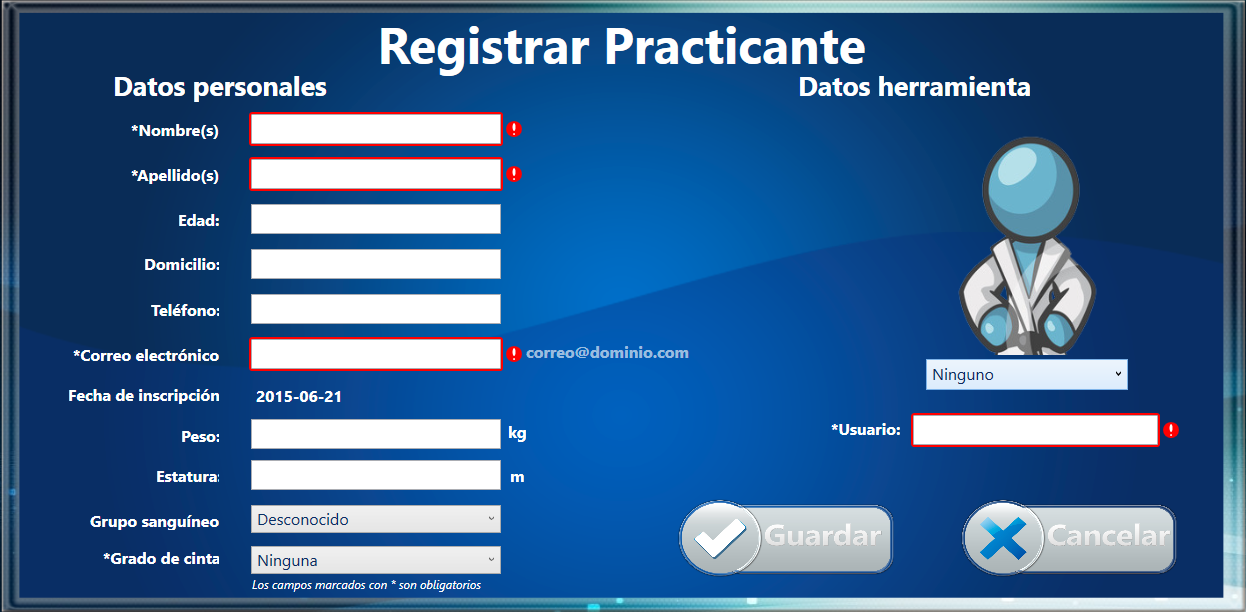
\includegraphics[scale=0.5]{./Figuras/Pantallas/IUE01Registrar_Practicante}
	\caption{IUE01 Registrar Practicante}
	\label{fig:IUE01}
\end{figure}

\textbf{\textcolor[rgb]{0, 0, 0.545098}{Entradas}}\\
En esta pantalla el Entrenador debe capturar la siguiente información:

\begin{itemize}
	\item El(Los) Nombre(s).
	\item El(Los) Apellido(s).
	\item La Edad.
	\item El Domicilio.
	\item El Teléfono.
	\item El Correo electrónico.
	\item El Peso del Practicante.
	\item La Estatura del Practicante.
	\item El nombre de Usuario del Practicante en la herramienta.
\end{itemize}
\vspace{1em}

\textbf{\textcolor[rgb]{0, 0, 0.545098}{Controles}}
\begin{itemize}
	\item \textbf{\textcolor[rgb]{0, 0, 0.545098}{Grupo sanguíneo:}} Permite seleccionar al Entrenador el grupo sanguíneo del Practicante que desea registrar.
	\item \textbf{\textcolor[rgb]{0, 0, 0.545098}{Grado de cinta:}} Permite seleccionar al Entrenador el grado de cinta del Practicante que desea registrar.
	\item \textbf{\textcolor[rgb]{0, 0, 0.545098}{Avatar del Practicante:}} Permite seleccionar al Entrenador un avatar para el Practicante que desea registrar.
\end{itemize}
\vspace{1em}

\textbf{\textcolor[rgb]{0, 0, 0.545098}{Comandos}}
\begin{itemize}
	\item \textbf{\textcolor[rgb]{0, 0, 0.545098}{Guardar:}} Permite al Entrenador registrar el nuevo Practicante cuando la información ingresada en los campos obligatorios sea correcta.
	\item \textbf{\textcolor[rgb]{0, 0, 0.545098}{Cancelar:}} Descarta la información registrada y muestra el menú \nameref{menu:ME02}.
\end{itemize}
\vspace{1em}

\textbf{\textcolor[rgb]{0, 0, 0.545098}{Mensajes}}\\

\textbf{\nameref{msj:MSG01}}: Se muestra en la pantalla \nameref{pant:IUE01} cuando el Entrenador haya registrado al Practicante en la herramienta de manera exitosa.\\

\textbf{\nameref{msj:MSG11}}: Se muestra en la pantalla \nameref{pant:IUE01} cuando el Entrenador intente registrar a un Practicante que ya se encuentre en la herramienta.\\

\textbf{\nameref{msj:MSG12}}: Se muestra en la pantalla \nameref{pant:IUE01} cuando el Entrenador no haya ingresado datos en alguno de los campos obligatorios.\\

\textbf{\nameref{msj:MSG13}}: Se muestra en la pantalla \nameref{pant:IUE01} cuando el Entrenador haya ingresado datos con un formato incorrecto en alguno de los campos.\\

\clearpage